\documentclass{article}
\usepackage{fullpage, amsmath, fancyvrb, graphicx, pgfplots}

\begin{document}

\section{Python}
\subsection{getting started with the code}
%This code can be used as a package either imported for use in a python script or in a terminal as follows: \\
\noindent\textbf{in a python script}:\\
Save your new python script in the folder \verb|flow_polytopes/|
at the top of it include the lines: 
\begin{Verbatim}
from graph_cal import *
from quiver_cal import *
\end{Verbatim}
Then use any of the functions listed below!
\vspace{.75cm}

\noindent\textbf{in a python shell}:\\
navigate to the folder \verb|flow_polytopes/|
\begin{Verbatim}
>>> from graph_cal import *
>>> from quiver_cal import *
\end{Verbatim}

\noindent\textbf{Building a first quiver}:\\
In python, the quiver $Q$ is represented using either a list of arrows 
$[(a_i, b_i)]$ for $a_i, b_i\in Q_0$, $i = 0, ..., |Q_1|$. 
or as a numpy matrix: 
$$\left[
a_{ij}=\begin{cases}
1,&\text{ if head of arrow }j\text{ is vertex }i\\
-1,&\text{ if tail of arrow }j\text{ is vertex }i\\
0,&\text{ otherwise }
\end{cases}
\right]$$
There is also funcionality to go between the two representations of a quiver, as shown below. 

\noindent\textbf{Example}: 
The code to represent the quiver shown below is given in two ways as a sample:\\
\vspace{.1cm}

\noindent\verb|sampleScipt.py|:\\
\vspace{.1cm}

\begin{minipage}{0.65\textwidth}
\begin{Verbatim}
from numpy import *
from graph_cal import *
from quiver_cal import *

Q_list = [(0,1),(0,2),(0,3),(4,1),(4,2),(4,3)]
Q_mat = matrix([
        [-1,-1,-1, 0, 0, 0],
        [ 1, 0, 0, 1, 0, 0],
        [ 0, 1, 0, 0, 1, 0],
        [ 0, 0, 1, 0, 0, 1],
        [ 0, 0, 0,-1,-1,-1]
        ])

\end{Verbatim}
\end{minipage}~
\begin{minipage}{0.3\textwidth}
	\resizebox{0.8\textwidth}{!}{
		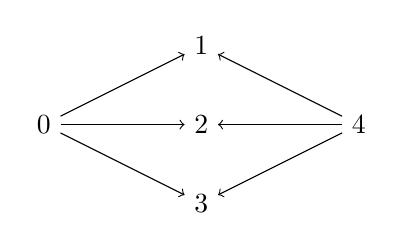
\begin{tikzpicture}
		\node[scale=1] (0) at (0, 0) {0};
		\node[scale=1] (1) at (2, 1) {1};
		\node[scale=1] (2) at (2, 0) {2};
		\node[scale=1] (3) at (2,-1) {3};
		\node[scale=1] (4) at (4, 0) {4};
                \draw[->] (0) -- (1);
                \draw[->] (0) -- (2);
                \draw[->] (0) -- (3);
                \draw[->] (4) -- (1);
                \draw[->] (4) -- (2);
                \draw[->] (4) -- (3);
		\end{tikzpicture}
	}
\end{minipage}

\subsection{available functions}
To obtain all $d$-dimensional quivers: 
\begin{Verbatim}
Qs = all_possible_graphs(d)
\end{Verbatim}
Get the polytope associated to the quiver $Q$: 
\begin{Verbatim}
flow_polytope(Q)
\end{Verbatim}
Generate all the subquivers of $Q$
\begin{Verbatim}
subquivers(Q)
\end{Verbatim}
Get all subsets of the vertices of $Q$ that are closed under arrows:
\begin{Verbatim}
subsets_closed(M)
\end{Verbatim}
Calculates weights of the vertices that are inherited from the weights on the arrows
\begin{Verbatim}
theta(Q)
\end{Verbatim}
Is the subquiver $subQ$ stable? 
\begin{Verbatim}
is_stable(Q, subQ)
\end{Verbatim}
\end{document}
